% Chapter Template

\chapter{Experiments} % Main chapter title

\label{Chapter4} % Change X to a consecutive number; for referencing this chapter elsewhere, use \ref{ChapterX}

\lhead{Chapter 4. \emph{Experiments}} % Change X to a consecutive number; this is for the header on each page - perhaps a shortened title

\section{Setup}

In order to see how the evoting service performs under load, we wanted to setup a set of nodes and simulate elections under different load. Since communication between the frontend and cothority happens over Websockets, a key requirement for the load testing framework was support for websockets. We chose Artillery \cite{artillery}, an extensible open source load testing framework written in Javascript. Artillery's extensibility allows us to write a custom \textit{engine} for it - \textit{artillery-engine-cothority} \cite{artillery-engine-cothority} which allows us to define load test scenarios that can use CothorityJS under the hood to communicate with the conodes.

\begin{figure}[htpb]
  \centering
    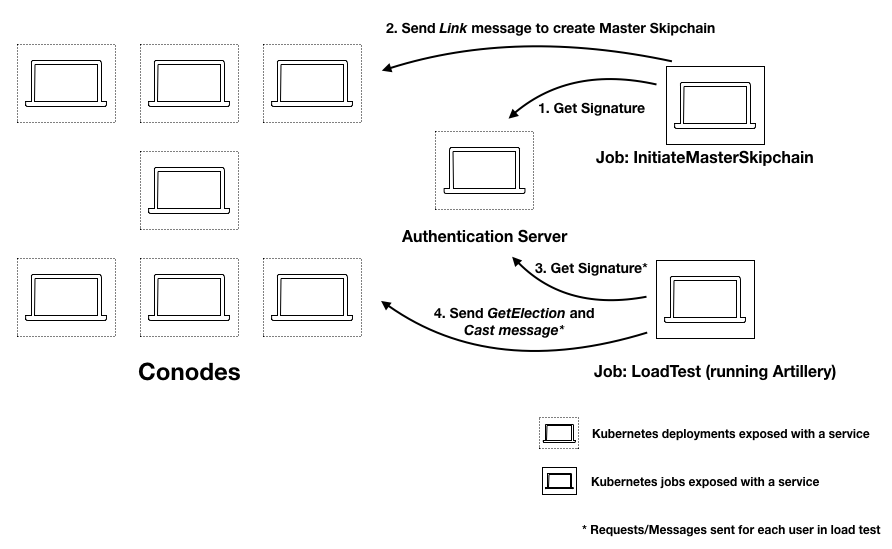
\includegraphics[scale=0.4]{Figures/Kubernetes.png}
    \rule{35em}{0.5pt}
  \caption[Loadtesting]{Loadtesting using Kubernetes and Artillery}
  \label{fig:Loadtesting}
\end{figure}


Next, to simulate our load tests, we used a Kubernetes Cluster provided by the IC Department at EPFL to orchestrate a set of Docker containers running the conodes, the authentication server and the load testing scripts. The end result is an easily configurable setup that allows load testing the evoting service at different transaction rates and different number of conodes. For our experiments, a transaction consists of sending a \textit{GetElection} message (to fetch the list of elections), followed by a \textit{Cast} message (to cast a ballot). This simulates the operations a user would do to cast their vote. The simulations were run with 7 conodes, each running in its own Kubernetes deployment at 2, 3 and 5 transactions per second.

\section{Optimisations}

Initial efforts to load test the evoting service lead to frequent timeouts and scaling issues while trying to fetch the list of elections or cast a ballot. As noted before, the evoting service uses skipchains to persist the transactions. Every block that is to be stored in the skipchain must be proposed by a \textit{leader}, which in case of the evoting application, happens to be the first node in the Election Roster. In an effort to allow all conodes to respond to messages sent by the frontend client, the evoting service in every non-leader node contacted the leader node over websockets to store a transaction. This resulted in a large number of network roundtrips which caused frequent timeouts and scaling issues.

An alternative to the above was to ensure that the frontend client may only communicate with the \textit{leader} which may propose a block using its local skipchain service and propagate it to other non-leader conodes. We therefore save on the network roundtrips in the previous scenario without adding new complexities to the system.

\section{Statistics}

\begin{figure}[!h]
\minipage[b]{0.5\textwidth}
    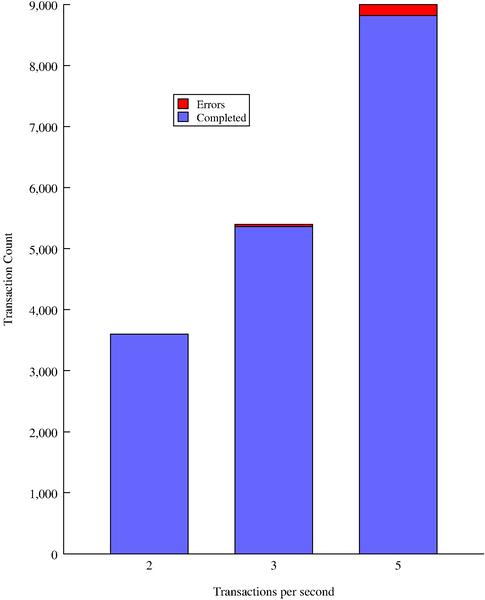
\includegraphics[width=\linewidth]{Figures/ScenarioResponses.png}
  \caption[Scenario Responses]{Scenario Responses}
  \label{fig:ScenarioResponses}
\endminipage\hfill
\minipage[b]{0.5\textwidth}
    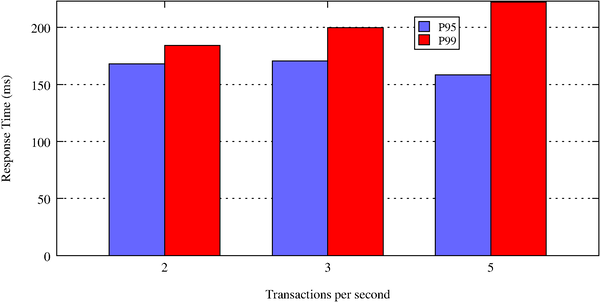
\includegraphics[width=\linewidth]{Figures/AggregateStats.png}
  \caption[Aggregate Statistics]{Aggregate Statistics}
  \label{fig:AggregateStats}
\endminipage\hfill
\end{figure}

After incorporating the optimisations mentioned above, we load tested the evoting service for a duration of 30 minutes at 2, 3 and 5 transactions per second. Figure \ref{fig:ScenarioResponses} shows a plot of the total transaction requests sent, and the proportion that succeeded and failed. We observe that at transaction rates of 2 and 3 TPS, the evoting system manages load fairly well and is quite responsive with 1 and 35 failures respectively. At 5 transactions per second the number of failures increase to 181 out of a total of 9000 transaction attempts.

Figure \ref{fig:AggregateStats} shows the P95 and P99 response times of the service at different loads. As expected response time increases as the service is exposed to a higher transaction rate but it still scales well at a P99 response time of 222.2ms at 5 transactions per second.  In another simulation at 3 transactions per second over 12 hours, the evoting service recorded 118,710 ballots with a P99 response time of 434.3ms.

These statistics indicate that the system should scale well in an Election at EPFL with about 10,000 voters in total. In practice, every department holds its separate election with a smaller list of eligible voters and the voting period being spread over 15 days.

\section{Resilience}

In a distributed architecture it is imperative for the system to be resilient and recover gracefully from node failures. Operations to the skipchain require ratification by \( \lfloor\dfrac{2n}{3}\rfloor + 1 \) nodes following the byzantine consensus requirement. As a result, we've kept the same threshold across all protocols used within evoting. The skipchain service in the conodes is resilient to downtime failures and tries to synchronise itself with the other nodes in the roster when it's available again. The initial implementation of the Shuffle and Decrypt protocols, however, were not resilient to node failures and timeouts and left the election skipchain in an invalid state in case of an error. This occurred because these protocols always assumed they began from a clean state, i.e. no previous attempts were made to Shuffle or Decrypt the election. Recent work on the project was to improve the resilience of these protocols by keeping track of the progress they made before failing, and whitelisting nodes to contact in every run of the protocol, filtering out the ones that have participated before in a previous attempt.